\chapter{Operational Semantics}

\section{Formal Properties}
\begin{center}
    \begin{tabular}{r l l}
        \textbf{Safety Properties} & \textit{Nothing bad happens} & Only violated by finite computations \\
        \textbf{Liveness Properties} & \textit{Something good happens eventually} & Cannot be violated by finite computation \\
    \end{tabular}
\end{center}
Deadlock is a \textbf{liveness} problem, while Mutual exclusion is a \textbf{Safety} problem.

\begin{definitionbox}{Communication Deadlock}
    When using transient communication, messages can be lost. 
    A thread may wait on a reply from another thread, that never 
    received to prompt to reply in the first place, thus causing a deadlock.
\end{definitionbox}

\begin{itemize}
    \item Mutual Exclusion cannot be solved with transient communication
    \item Interrupts can also not work?
\end{itemize}

\begin{definitionbox}{Mutual Exclusion}
    When only one thread can execute in a critical region at a time, there is mutual exclusion.
    \begin{itemize}
        \item Mutual exclusion enforces removes parallelism for the critical section, limiting speedup from parallelism (Amdahl's law)
    \end{itemize}
\end{definitionbox}

\begin{tcbraster}[raster columns=2, raster equal height]
    \begin{definitionbox}{Turing Computability}
        A model of computation that describes what is computable. 
        \begin{itemize}
            \item Efficiency mostly irrelevant
            \item Only covers sequential computation.
        \end{itemize}
    \end{definitionbox}
    \begin{definitionbox}{Shared-Memory Computability}
        A model for concurrent computation.
        \begin{itemize}
            \item Describes what is concurrently computable.
            \item Efficiency mostly irrelevant
        \end{itemize}
    \end{definitionbox}
\end{tcbraster}

\section{Shared-Memory Concurrency}
\subsection{Read-Modify-Write}
\begin{definitionbox}{Read-Modify-Write Instructions}
    An instruction that reads, modifies (with some function) and writes to a memory location, returning the value prior to the modification.
    \begin{minted}{Rust}
//! Generically we can express this scheme for any data type
struct RMWLocation<A> {data: A}

impl<A: Clone> RMWLocation<A> {
    /// This function is synchronised
    fn read_modify_write(&mut self, apply: fn(&A) -> A) -> A {
        let old_value = self.data.clone();
        self.data = apply(&self.data);
        old_value
    }
}
    \end{minted}
\end{definitionbox}
There are many different RMW instructions, a read can be considered an RMW instruction (where modification applies is just identity).
\begin{tcbraster}[raster columns=2, raster equal height]
    \begin{definitionbox}{Weak RMW}
        Allows for synchronisation between two threads.
        \begin{itemize}
            \item exchange Write - a new value to the location.
            \item fetch and add - Atomically add to an integer at a location. \\
        \end{itemize}
    \end{definitionbox}
    \begin{definitionbox}{Strong RMW}
        Allows for synchronisation between an arbitrary number of threads.
        \begin{itemize}
            \item compare and set (CAS) - If the value is equal to the expected, set to updated and return true, else return false.
        \end{itemize}
    \end{definitionbox}
\end{tcbraster}
Many early machines provided weak RMW instructions (Test-and-set in IBM 360, Swap in original SPARCs), we now understand the limitations of these.
\begin{itemize}
    \item All intel x86 architectures support CAS.
    \item ARM supports CAS through through load-linked and store-conditional instructions.
\end{itemize}

\subsection{Consistency/Memory Models}
\begin{definitionbox}{Sequential Consistency}
    Also known as interleaving semantics.
    \begin{itemize}
        \item Instructions for each thread are executed in order.
        \item Instructions from different threads can be interleaved arbitrarily.
    \end{itemize}
\end{definitionbox}
\subsubsection{Sequential Consistency Model}
\begin{itemize}
    \item Can work on a uniprocessor system (simple/idealised).
    \item A good abstraction for concurrency \& easier to reason about.
    \item Not available on any hardware platform by default.
    \item Inefficient and expensive to implement.
\end{itemize}
\subsubsection{Hardware Consistency Models}
\begin{itemize}
    \item A weak memory model (due to dynamic scheduling on processors)
    \item Complex for multicore systems.
    \item Hardware implementation has to deal with complexities such as cache coherence.
\end{itemize}
\subsubsection{Software/Programming Language Consistency Models}
\begin{itemize}
    \item A weak memory model (compiler can reorder instructions, also must accommodate hardware)
    \item Determined by the language specification, programmer uses this specification, compiler adapts to hardware.
    \item C/C++ 2011 model (C11 model) (e.g \mintinline{C}{atomic.h})
    \item Java Memory Model
\end{itemize}

\section{Sequential Consistency}
We can create a basic while-language for sequential consistency.
\[\begin{matrix}
    B \in Bool ::= \dots & E \in Exp::= \dots & \wmem{x}, \wmem{y}, \wmem{x} \dots \in Loc ::= \text{ (Memory Location)} & \wreg{a}, \wreg{b}, \wreg{c} \dots \in Reg ::= \text{ (Register)} \\
\end{matrix}\]

\[\begin{split}
    C \in Com ::= &\  \wass{\wreg{a}}{E} \\
    | & \  \wass{\wreg{a}}{\wmem{x}} \\
    | & \  \wass{\wmem{x}}{\wreg{a}} \\
    | & \  \wass{\wreg{a}}{\wcas{\wmem{x}}{E}{E}}\\
    | & \  \wffa{\wmem{x}}{E} \\
    | & \  \wskip \\
    | & \  \wseq{C}{C} \\
    | & \  \wwhile{B}{C} \\
    | & \  \wif{B}{C}{C} \\
\end{split}\]

Concurrent programs are modelled as a map from thread identifiers to sequential commands.
\[\begin{matrix}
    \tau \in Tid & \text{  and  } & P \in Prog \triangleq Tid \rightarrow Com
\end{matrix}\]
A concurrent program can be expressed using $||$ as:
\[C_1 || C_2 || C_3 || \dots || C_n \text{ for program } P \text{ where } dom(P) = \{\tau_1, \tau_2, \tau_3, \dots, \tau_n\} \text{ and } P(\tau_i) = C_i \text{ for } i \in \{1,2,3,\dots, n\} \]
\begin{examplebox}{Racey Increment}
    Write a concurrent program $\text{inc}$ that comprises of two threads which increment some shared memory.
    \tcblower
    \[P_{\text{inc}} \triangleq \left. \begin{matrix*}[l]
        \wass{\wreg{a1}}{cnt} \\
        \wass{\wreg{a1}}{\wreg{a1} + 1} \\
        \wass{\wmem{cnt}}{\wreg{a1}} \\
    \end{matrix*} \ \right\lvert \left\rvert \
    \begin{matrix*}[l]
        \wass{\wreg{a2}}{cnt} \\
        \wass{\wreg{a2}}{\wreg{a2} + 1} \\
        \wass{\wmem{cnt}}{\wreg{a2}} \\
    \end{matrix*} \right.\]
    We can also express this as:
    \[dom(P_{\text{inc}}) = \{\tau_1, \tau_2\} \begin{split}
        P_{\text{inc}}(\tau_1) &= \wseq{
            \wass{\wreg{a1}}{cnt} 
        }{\wseq{
            \wass{\wreg{a1}}{\wreg{a1} + 1} 
        }{
            \wass{\wmem{cnt}}{\wreg{a1}} 
        }} \\
        P_{\text{inc}}(\tau_1) &=  \wseq{
            \wass{\wreg{a2}}{cnt} 
        }{\wseq{
            \wass{\wreg{a2}}{\wreg{a2} + 1} 
        }{
            \wass{\wmem{cnt}}{\wreg{a2}} 
        }} \\
    \end{split}\]
\end{examplebox}

\subsection{Configurations}
\[\begin{split}
    \text{Shared memory } & M \in Mem \triangleq Loc \to Val \\
    \text{Thread-local Registers } & s \in Store \triangleq Reg \to Val \\
    \text{A store map for threads } & S \in SMap \triangleq Tid \to Store  \text{ where } S(\tau) = s \\
\end{split}\]
Hence the configuration is a triple of the concurrent program, shared memory and map to thread local stored.
\[(P, S, M)\]

\subsection{Transitions}
The operational semantics are split into two types of transition.
\begin{center}
    \begin{tabular}{l p{.8\textwidth}}
        \textbf{Program Transitions} & A step in program execution (e.g if condition) \\
        \textbf{Storage Transitions} & Describes behaviour of memory (e.g read/write) \\
    \end{tabular}
\end{center}
\begin{itemize}
    \item By splitting operational semantics into two parts we can alter storage transitions later without having to change the program transitions.
    \item The program and storage transitions are combined through label transitions.
\end{itemize}

The labels are defined as:
\[\begin{matrix*}[l]
    l \in Lab ::= & \ \ \epsilon         & \text{empty label such as when transitioning: } \wseq{\wskip}{C} \to C \\
                & | \ (R, \wmem{x}, v) & \text{Read value }v\text{ from memory location } \wmem{x} \\
                & | \ (W, \wmem{x}, v) & \text{Write value }v\text{ to memory location } \wmem{x} \\
                & | \ (U, \wmem{x}, v_0, v_n) & \text{Successful update of }\wmem{x}\text{ from }v_0 \to v_n \text{ (FFA or successful CAS)} \\
                & | \ (U, \wmem{x}, v_0, \bot) & \text{Failed CAS of }\wmem{x}\text{ where the old value of }\wmem{x}\text{ was not }v_0 \\
\end{matrix*}\]
We also have a total function $\ceval{s}{E}$ or $\ceval{s}{B}$ to evaluate expressions.
\begin{definitionbox}{Total Function}
    A function defined for all possible input values.
\end{definitionbox}
\noindent Hence any transition is:
\[C, s \ctrans{l} C',s' \text{ where } C, C' \in Com, \quad s, s' \in Store \text{ and } l \in Lab\]
The transitions are:
\\ \begin{minipage}{.33\textwidth}
    \[\cfrac{
    C_1, s \ctrans{l} C_1', s'
    }{
    \wseq{C_1}{C_2}, s \ctrans{l} \wseq{C_1'}{C_2}, s'
    }\]
    
\end{minipage}
\begin{minipage}{.33\textwidth}
    \[\cfrac{
        \ceval{s}{B} = true
    }{
        \wif{B}{C_1}{C_2},s \ctrans{\epsilon} C_1, s
    }\]
    \[\cfrac{
        \ceval{s}{B} = false
    }{
        \wif{B}{C_1}{C_2},s \ctrans{\epsilon} C_2, s
    }\]
\end{minipage}
\begin{minipage}{.33\textwidth}
    \[\cfrac{}{
        \wseq{\wskip}{C}, s \ctrans{\epsilon} C, s
    }\]
    \[\cfrac{
        \ceval{s}{E} = v \quad s' = s[\wreg{a} \mapsto v]
    }{
        \wass{\wreg{a}}{E}, s \ctrans{\epsilon} \wskip, s'
    }\]
\end{minipage}
\[\cfrac{}{
    \wwhile{B}{C},s \ctrans{\epsilon} \wif{B}{(\wseq{C}{\wwhile{B}{C}})}{skip}
}\]
We must also consider the basic read/write transitions:
\\ \begin{minipage}{.5\textwidth}
    \[\cfrac{
        s(\wreg{a}) = v
    }{
        \wass{\wmem{x}}{\wreg{a}} \ctrans{(W, \wmem{x}, v)} skip, s
    }\]
\end{minipage}
\begin{minipage}{.5\textwidth}
    \[\cfrac{
        s' = s[\wreg{a} \mapsto v]
    }{
        \wass{\wreg{a}}{\wmem{x}}, s \ctrans{(R, \wmem{x}, v)} skip, s'
    }\]
\end{minipage}
Note that program transitions do not consider memory, so no update takes place here on the memory write.
\\
\\ Finally we need to consider FFA and CAS.
\\ \begin{minipage}{.5\textwidth}
    \[\cfrac{
        \ceval{s}{E} = v \quad v_n = v_0 + v
    }{
        \wffa{\wmem{x}}{E},s \ctrans{(U, \wmem{x}, v_0, v_n)} skip, s
    }\]
\end{minipage}
\begin{minipage}{.5\textwidth}
    \[
        \cfrac{
            \ceval{s}{E_0} = v_0 \quad \ceval{s}{E_n} = v_n \quad s' = s[\wreg{a} \mapsto 1]
        }{
            \wass{\wreg{a}}{\wcas{\wmem{x}}{E_0}{E_n}}, s \ctrans{(U, \wmem{x}, v_0, v_n)} \wskip, s'
        }
    \]
    \[
        \cfrac{
            \ceval{s}{E_0} = v_0 \quad v \neq v_0 \quad s' = s[\wreg{a} \mapsto 0]
        }{
            \wass{\wreg{a}}{\wcas{\wmem{x}}{E_0}{E_n}}, s \ctrans{(U, \wmem{x}, v, \bot)} \wskip, s'
        }
    \]    
\end{minipage}



\subsection{Concurrent Program Transitions}
\[\cfrac{
    P(\tau) = C \quad S(\tau) = s \quad C,s \ctrans{l} C', s' \quad P' = P[\tau \mapsto C'] \quad S'=S[\tau \mapsto s']
}{
    P, S \ptrans{\tau}{l} P', S'
}\]

\subsection{Storage Transitions}
A storage transition is of the form $M \mtrans{\tau}{l} M'$ (thread $\tau$ updates $M \to M'$ using label $l$).
\begin{itemize}
    \item We will use the thread id $\tau$ to combine storage with program transitions later.
    \item We only consider the labels from program transitions (these affect the shared memory).
\end{itemize}
\begin{minipage}{.33\textwidth}
    \[\cfrac{
        M(\wmem{x}) = v
    }{
        M \mtrans{\tau}{(R, \wmem{x}, v)} M
    }\]
    \centerline{Memory Read}
\end{minipage}
\begin{minipage}{.33\textwidth}
    \[\cfrac{
        M' = M[\wmem{x} \mapsto v]
    }{
        M \mtrans{\tau}{(W \wmem{x}, v)} M'
    }\]
    \centerline{Memory Write}
\end{minipage}
\begin{minipage}{.33\textwidth}
    \[\cfrac{
        M(x) = v_0 \quad M' = M[\wmem{x} \mapsto v_n]
    }{
        M \mtrans{\tau}{(U, \wmem{x}, v_0, v_n)} M'
    }\]
    \centerline{Successful CAS or FFA}
\end{minipage}
\vspace{5mm}
\\ \begin{minipage}{.33\textwidth}
    \[\cfrac{
        M(\wmem{x}) = v
    }{
        M \mtrans{\tau}{(U, \wmem{x}, v, \bot)} M
    }\]
    \centerline{Failed CAS}
\end{minipage}

\subsection{Combining Operational Semantics}
The combined semantics are of the form $P, S, M \to P', S', M'$
\\
\\ For example with 
\[\cfrac{
    P, S \ptrans{\tau}{\epsilon} P', S'
}{
    P, S, M \to P' S', M
}\]
\centerline{Under $\epsilon$ label shared memory is unchanged}
\\
If the program and storage transitions are the same, then we can combine into a single transition
\begin{examplebox}{Skipping it!}
    Combine the memory and program transitions for skip.
    \tcblower
    The program transition can be expressed as:
    \[\cfrac{
        P(\tau) = \wseq{\wskip}{C} \quad S(\tau) = s \quad \wseq{\wskip}{C}, s \ctrans{\epsilon} C,s \quad P' = P[\tau \mapsto C]    
    }{
        P, S \ptrans{\tau}{\epsilon} P', S
    }\]
    As the program transition does not affect memory ($\wseq{\wskip}{C}, s \ctrans{\epsilon} C,s$) we can directly add $M$ to the transition:
    \[\cfrac{
        P(\tau) = \wseq{\wskip}{C} \quad S(\tau) = s \quad \wseq{\wskip}{C}, s \ctrans{\epsilon} C,s \quad P' = P[\tau \mapsto C]    
    }{
        P, S, M \to P', S, M
    }\]
\end{examplebox}
\begin{examplebox}{Read and Assign}
    Get the program transition for an assignment (reading memory into a register), where the memory value is $7$.
    \tcblower
    \begin{minipage}{.5\textwidth}
        \[\cfrac
        {
            M(\wmem{x}) = 7
        }{
            M \mtrans{\tau}{(R, \wmem{x}, 7)} M
        }
    \]    
    \end{minipage}
    \begin{minipage}{.5\textwidth}
    \[\cfrac{
        s' = s[\wreg{a} \mapsto 7]
    }{
        \wass{\wreg{a}}{\wmem{x}}, s \ctrans{(R, \wmem{x}, 7)} \wskip, s'
    }\]
    \end{minipage}
    
    \[\cfrac{
        P(\tau) = \wass{\wreg{a}}{\wmem{x}} \quad S(\tau) = s \quad s' = s[\wreg{a} \mapsto 7] \quad \wass{\wreg{a}}{\wmem{x}},s \ctrans{(R, \wmem{x}, 7)} \wskip, s' \quad P' = P[\tau \mapsto \wskip] \quad S' = S[\tau \mapsto s']
    }{
        P,S \ptrans{\tau}{(R, \wmem{x}, 7)} P', S'
    }\]
    Hence we can now include the storage transition:
    \[\cfrac{
        P,S \ptrans{\tau}{(R, \wmem{x}, 7)} P', S' \quad M \mtrans{\tau}{(R, \wmem{x}, 7)} M
    }{
        P, S, M \to P', S', M
    }\]
\end{examplebox}

\subsection{Traces}
\begin{definitionbox}{$\to^*$ for SC}
    \[P, S, M \to^* P', S', M' \Leftrightarrow \begin{matrix*}[l]
        (P,S,M) = (P',S',M') \\
        \lor \exists (P'', S'', M'') . [P, S, M \to P'', S'', M'' \land P'', S'', M'' \to^* P', S', M'] \\
    \end{matrix*}\]
    The reflexive, transitive closure of $\to$
\end{definitionbox}

\begin{itemize}
    \item \textit{Initial memory} is all zeros $M_0 \triangleq \lambda x . 0$ (for any $x$, $M_0(x) = 0$).
    \item \textit{Initial Store} is also originally all zeros. $s_0 \triangleq \lambda a. 0$.
    \item \textit{Initial store map} is $S_0 \triangleq \lambda \tau . s_0$
    \item \textit{Terminated Program} is $P_{\wskip}$ expressed as $P_{\wskip} \triangleq \tau. \wskip$ .
    \item The \textit{initial configuration} is $(P, S_0, M_0)$.
\end{itemize}
Given a program $P$ the \textit{SC-trace} is the evaluation path:
\[P, S_0, M_0 \to^* P_{\wskip}, S, M\]
Where $(S, M)$ is the \textit{SC-outcome} of program $P$.

\subsection{Properties of Sequential Consistency}
\subsubsection{Determinism}
\[\forall P, P_1, P_2, S, S_1, S_2 M, M_1, M_2 . [
    (P,S,M \to P_1, S_1, M_1 \land P, S, M \to P_2, S_2, M_2)
    \Rightarrow
    ((P_1, S_1, M_1) = (P_2, S_2, M_2))
] \]
This does not hold due to the interleavings of the threads of $P$.
\begin{examplebox}{It has been determined\dots}
    Provide a counter example to SC being deterministic and confluent.
    \tcblower
    \[P = \left.\begin{matrix*}[l]
        \wass{\wreg{a1}}{1} \\
        \wass{\wmem{x}}{\wreg{a1}}
    \end{matrix*} \right| \left| \begin{matrix*}[l]
        \wass{\wreg{a2}}{0} \\
        \wass{\wmem{x}}{\wreg{a2}}
    \end{matrix*}\right.\]
    Here we can have $P, S_0, M_0 \to^* P_{\wskip}, S, M$ Where $M(\wmem{x}) = 1]$ or $M(\wmem{x}) = 0$.
\end{examplebox}

\subsubsection{Confluence}
\begin{multline*}
    \forall P, P_1, P_2, S, S_1, S_2 M, M_1, M_2 . [(P, S, M \to^* P_1, S_1, M_1 \land P, S, M \to^* P_2, S_2, M_2) 
    \\ \Rightarrow \exists P', S', M' . [P_1, S_1, M_1 \to^* P', S', M' \land P_2, S_2, M_2 \to^* P', S', M']]  
\end{multline*}
SC is not confluent for the same reason it is not deterministic (there are many possible \textit{SC-outcomes} for a program)

\section{Total Store Ordering}
\begin{definitionbox}{Weak Memory Models (WMM)}
    Allow for instructions in a thread to be reordered (e.g dynamically scheduled processors).
    \begin{itemize}
        \item \textit{Weak behaviours} are states not observable under \textit{sequential consistency}.
        \item Used by virtually all computer architectures (e.g TSO used by x86).
    \end{itemize}
\end{definitionbox}
\begin{definitionbox}{Total Store Ordering (TSO)}
    A weak memory model that allows for write-read reordering between different memory locations.
    \begin{itemize}
        \item A later read on $y$ can be reordered before an earlier write on $x$ when $x \neq y$
        \item Includes the interleaving semantics from sequential consistency.
        \item Allows for weak store buffering (where )
    \end{itemize}
\end{definitionbox}

\begin{center}
    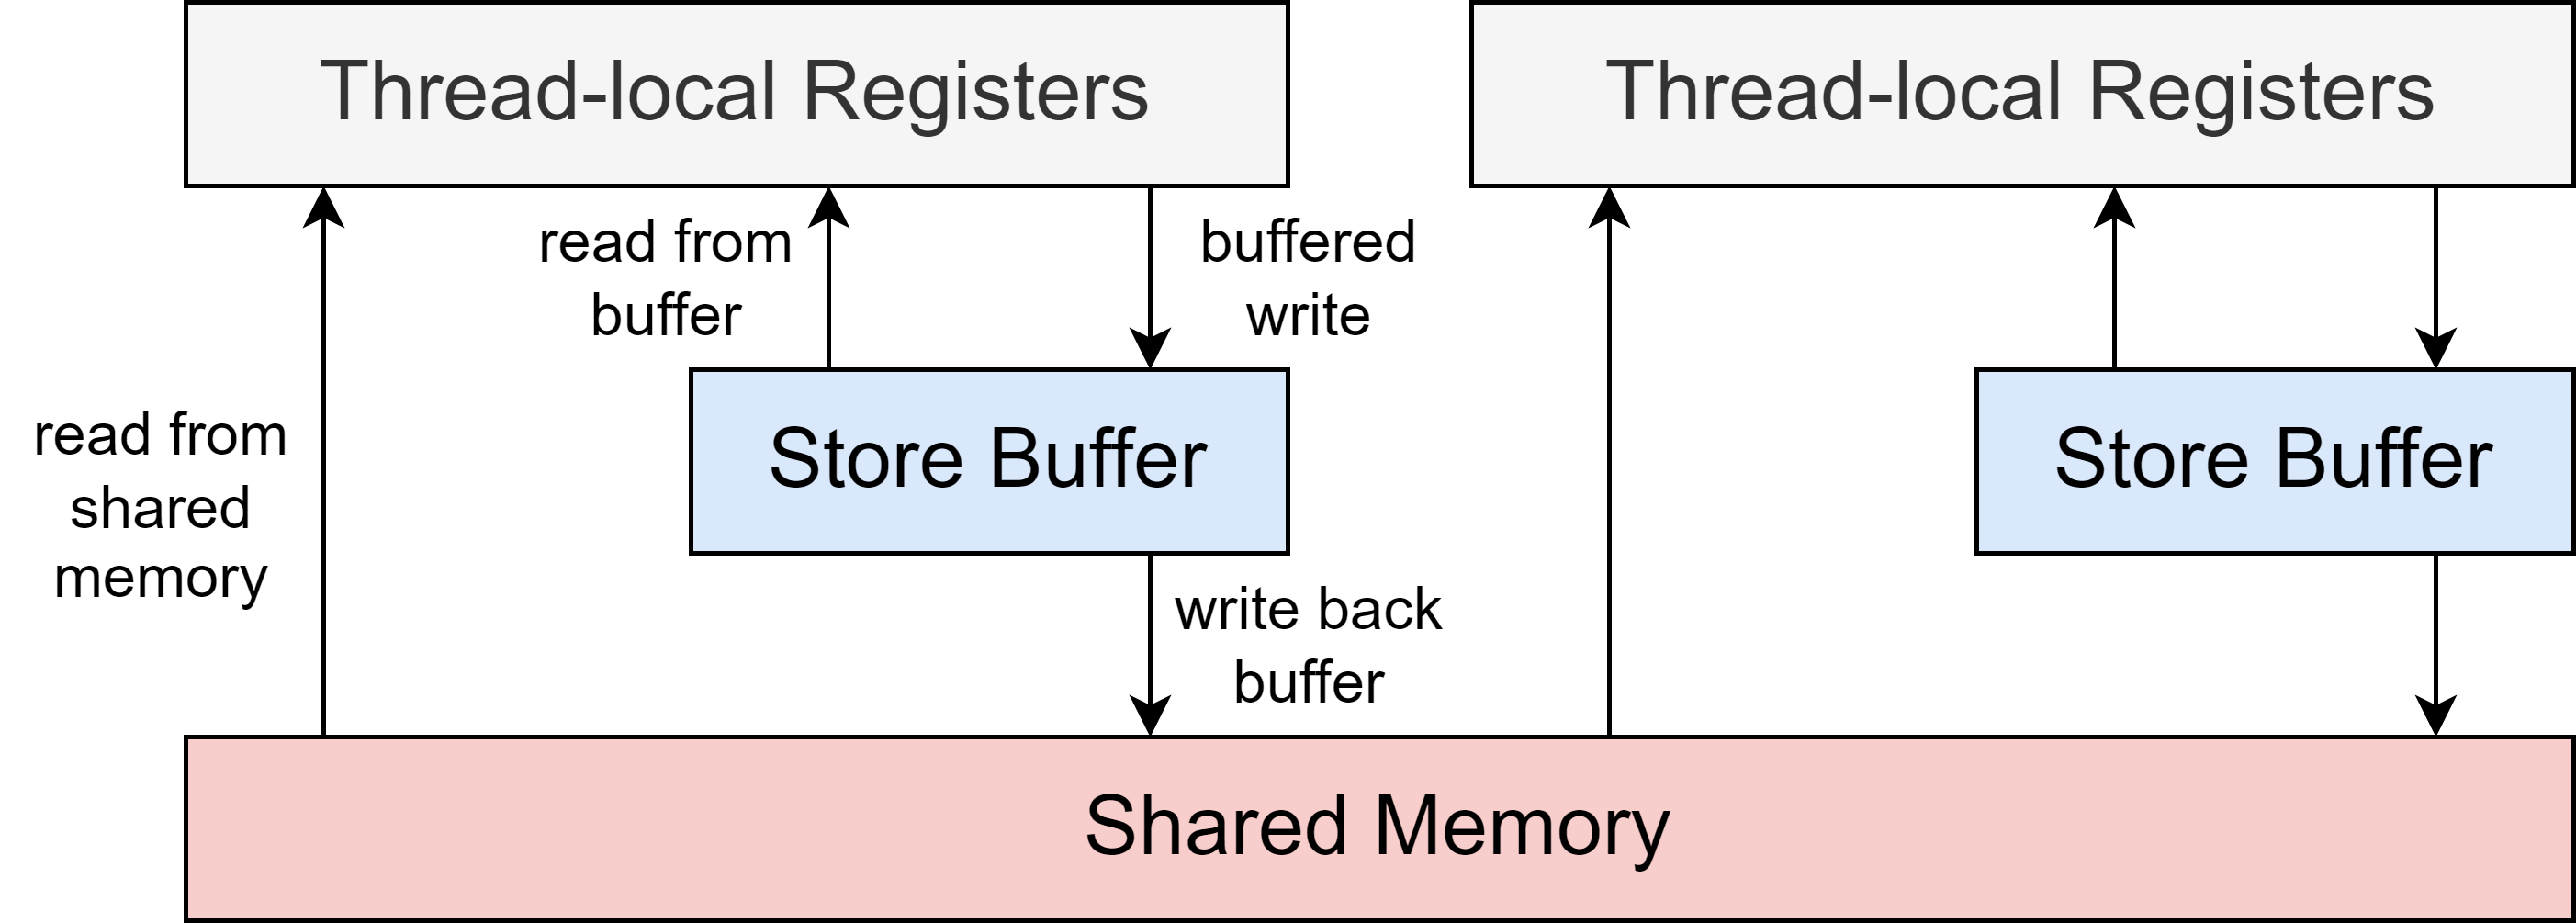
\includegraphics[width=.8\textwidth]{operational_semantics/images/tso.drawio.png}
\end{center}
\begin{center}
    \begin{tabular}{l p{.8\textwidth}}
        $\wass{\wmem{x}}{1}$ & Add $\wass{\wmem{x}}{1}$ to the store buffer. \\
        $\wass{\wreg{a}}{\wmem{x}}$ & If $\wmem{x}$ is in the buffer, read latest entry, else read from shared memory. \\
        unbuffer & Flush buffer to memory (FIFO order) \\
        $\wmfence$ & Barrier instruction, ensures no delayed writes are in the buffer (hence any subsequent reads happen after the current buffered writes). \\
        RWMs & Act as barriers and ensure no delayed writes are in the buffer, they write directly to memory without delay. \\
    \end{tabular}
\end{center}

The previous language used for sequential consistency can have fences added.
\[\begin{split}
    C \in Com ::= &\  \wass{\wreg{a}}{E} \\
    | & \  \wass{\wreg{a}}{\wmem{x}} \\
    | & \  \wass{\wmem{x}}{\wreg{a}} \\
    | & \  \wass{\wreg{a}}{\wcas{\wmem{x}}{E}{E}}\\
    | & \  \wffa{\wmem{x}}{E} \\
    | & \  \wskip \\
    | & \  \wseq{C}{C} \\
    | & \  \wwhile{B}{C} \\
    | & \  \wif{B}{C}{C} \\
    | & \  \wmfence \\
\end{split}\]

\[\cfrac{}{
        \wmfence, s \ctrans{MF} \wskip, s
    }\]

We model memory similarly to before, but now with a local buffer.
\[M \in Mem \triangleq Loc \to Val \qquad S \in SMap \triangleq Tid \to Store \qquad s \in Store \triangleq Reg \to Val\]
A buffer is a FIFO queue of delayed write labels.
\[b \in Buff \triangleq Seq\langle WLab \rangle \qquad Wlab \triangleq \{(W, \wmem{x}, v) | x \in Loc \land v \in Val\}\]
\[B \in BMap \triangleq Tid \to Buff \text{ where } b = B(\tau)\]

Hence a TSO configuration is:
\[(P, S, M, B)\]

\subsection{Storage Transitions}
TSO adds the $\wmfence$ transition label $MF$
\[\begin{split}
    l \in Lab ::= & \ \epsilon \\
    | & \ (R, \wmem{x}, v) \\
    | & \ (W, \wmem{x}, v) \\
    | & \ (U, \wmem{x}, v_0, v_n) \\
    | & \ (U, \wmem{x}, v_0, \bot) \\
    | & \ MF \\
\end{split}\]
Storage transitions are of the form:
\[M, B \mtrans{\tau}{l} M', B'\]
\begin{minipage}[b]{.5\textwidth}
    \[\cfrac{
        B(\tau) = b \quad b' = b.(W, \wmem{x}, v) \quad B' = B[\tau \mapsto b']
    }{
        M,B \mtrans{\tau}{(W, \wmem{x}, v)} M,B'
    }\]
    \centerline{Memory Write}
\end{minipage}
\begin{minipage}[b]{.5\textwidth}
    \[\cfrac{
        B(\tau) = b \quad get(M, b, \wmem{x}) = v
    }{
        M, B \mtrans{\tau}{(R, \wmem{x}, v)} M, B
    }\]
    \[get(M, b, \wmem{x}) \triangleq \begin{cases}
        v & \begin{matrix*}[l]
            \text{if } \exists b_1, b_2. [b = b_1.(W, \wmem{x}, v).b_2] \\ 
            \land \neg\exists v'. [(W, \wmem{x}, v') \in b_2] \\
        \end{matrix*} \\
        M(x) & \text{otherwise} \\
    \end{cases} \]
    \centerline{Memory Read}
\end{minipage}
\\ \begin{minipage}[b]{.33\textwidth}
    \[\cfrac{B(\tau) = \emptyset}{M,B \mtrans{\tau}{MF}M, B}\]
    \centerline{Memory Fence ensures no buffering}
\end{minipage}
\begin{minipage}[b]{.33\textwidth}
    \[\cfrac{
        B(\tau) = \emptyset \quad M(\wmem{x}) = v_0 \quad M' = M[\wmem{x} \mapsto v_n]
    }{
        M, B \mtrans{\tau}{(U, \wmem{x}, v_0, v_n)} M' B
    }\]
    \centerline{Successful RMW}
\end{minipage}
\begin{minipage}[b]{.33\textwidth}
    \[\cfrac{
        B(\tau) = \emptyset \quad M(\wmem{x}) = v
    }{
        M, B \mtrans{\tau}{(U, \wmem{x}, v, \bot)} M B
    }\]
    \centerline{Failed RMW}
\end{minipage}
\vspace{5mm}
The buffered writes may be propagated at any time through a silent step, this is done using an $\epsilon$ storage transition.
\[\cfrac{
    B(\tau) = (W, \wmem{x}, v).b \quad M' = M[\wmem{x} \mapsto v] \quad B' = B[\tau \mapsto b]
}{
    M, B \mtrans{\tau}{\epsilon} M', B'
}\]

\begin{minipage}[b]{.48\textwidth}
    \[\cfrac{
    P, S \ptrans{\tau}{\epsilon} P', S'
    }{
        P, S, M, B \to P', S', M, B
    }\]
    If the program takes a silent step, the storage system is unchanged.
\end{minipage}
\hfill
\vline
\hfill
\begin{minipage}[b]{.45\textwidth}
    \[\cfrac{
        M, B \mtrans{\tau}{\epsilon} M', B'
    }{
        P, S, M, B \to P, S, M', B'
    }\]
    If the storage system takes a silent step, the program \& program's register store remains the same.
\end{minipage}
\vspace{5mm}
If both the program and storage systems make the same transition $l$ then we can combine this into a transition over the TSO configuration.
\[\cfrac{
    P, S \ptrans{\tau}{l} P', S' \qquad M, B \mtrans{\tau}{l} M', B'
}{
    P, S, M, B \to P', S', M', B'
}\]

\begin{examplebox}{sFence}
    The x86-64 instruction set includes an $\wsfence$ instruction. This is similar to $\wmfence$, however allows for read reordering.
    \[ \begin{matrix}
        \left. \begin{matrix*}[l]
            \wass{\wmem{x}}{1} \\
            \wsfence \\
            \wass{\wreg{a}}{\wmem{y}} \\
        \end{matrix*}\right\lVert \begin{matrix*}[l]
            \wass{\wmem{y}}{1} \\
            \wsfence \\
            \wass{\wreg{b}}{\wmem{x}} \\
        \end{matrix*} \\
        \text{Original}
    \end{matrix}
    \quad \approx \quad 
    \begin{matrix}
        \left. \begin{matrix*}[l]
            \wass{\wmem{x}}{1} \\
            \wass{\wreg{a}}{\wmem{y}} \\
            \wsfence \\
        \end{matrix*}\right\lVert \begin{matrix*}[l]
            \wass{\wmem{y}}{1} \\
            \wass{\wreg{b}}{\wmem{x}} \\
            \wsfence \\
        \end{matrix*} \\
        \wsfence\text{-read-reordering}
    \end{matrix}
    \quad \approx \quad 
    \begin{matrix}
        \left. \begin{matrix*}[l]
            \wass{\wreg{a}}{\wmem{y}} \\
            \wass{\wmem{x}}{1} \\
            \wsfence \\
        \end{matrix*}\right\lVert \begin{matrix*}[l]
            \wass{\wreg{b}}{\wmem{x}} \\
            \wass{\wmem{y}}{1} \\
            \wsfence \\
        \end{matrix*} \\
        \text{TSO allowed reorder}
    \end{matrix}\]
    Adapt the rules of TSO to implement $\wsfence$.
    \tcblower
    $\wsfence$ make no changes to registers/local store, but requires an $SF$ memory transition:
    \[\cfrac{}{
        \wsfence, s \ctrans{SF} \wskip, s
    }\]
    \\
    \\ In order to implement, we will add $\wsfence$s to the store buffer, hence we must redefine the buffer:
    \[b \in Buff \triangleq Seq \langle WLab \cup \{SF\}\rangle\]

    \begin{itemize}
        \item $\wsfence$ adds $SF$ to the store buffer.
        \item When executing an $\wsfence$ transition, we do not need to check if the buffer is empty.
        \item Since $\wsfence$ and write instructions are still ordered with respect to eachother, the buffers are still a FIFO queue.
    \end{itemize}
    Hence:
    \\ \begin{minipage}{.5\textwidth}
        \[\cfrac{
            B(\tau) = b \quad B' = B[\tau \mapsto b.SF]
        }{
            M, B \mtrans{\tau}{SF} M, B'
        }\]
    \end{minipage}
    \begin{minipage}{.5\textwidth}
        \[\cfrac{
            B(\tau) = SF.b \quad B' = B[\tau \mapsto b]
        }{
            M, B \mtrans{\tau}{\epsilon} M, B'
        }\]
    \end{minipage}
    We can consider an $\wsfence$ as a kind of dummy write, much like normal writes other writes cannot be reordered, but reads can. However unlike a write it has no effect on memory.
\end{examplebox}

\subsection{Traces}
TSO inherits much of the initial state from SC:
\[M_0 \triangleq \lambda x . 0 \qquad S_0 \triangleq \lambda \tau . s_0 \text{ with } s_0 \triangleq \lambda a . 0 \qquad P_{\wskip} \triangleq \lambda \tau. \wskip\]
However we add the \textit{initial buffer map}:
\[B_0 \triangleq \lambda \tau . \emptyset\]
The \textit{initial TSO-configuration} is hence:
\[(P, S_0, M_0, B_0)\]
Given some program $P$ the \textit{TSO-trace} is an evaluation path that starts from the \textit{initial TSO-configuration} of $P$ and terminates with $P_{\wskip}$ and empty buffers.
\[P, S_0, M_0, B_0 \to^* P_{\wskip}, S, M, B_0 \text{ where } (S, M) \text{ is the \textit{TSO-outcome}}\]

\subsection{Properties of Total Store Ordering}
\subsubsection{Determinism}
Much like \textit{sequential consistency} the interleaving of different threads makes TSO non-deterministic.

\subsubsection{Confluence}
Likewise, TSO is not confluent.